\subsection{QLS Code Generator}

So far, our QLS models have no effect on the generated output. The first step
is to think about which artifacts are to be generated from a QLS model. The QLS
model contains two kinds of information. The first is layout information: A page
consists of one or more forms. Recall that for each form two XHTML files are
already generated, one for the base content of the form site and a wrapper
referencing this base XHTML. Hence a page maps to an XHTML file which is
composed of all specified forms. The second information in QLS is styling
information. As usual in web development, styling is expressed in the CSS format
in our tool. To sum up:

For each page:
\begin{itemize}
  \item Generate one CSS file
  \item Generate one XHTML file wiring all form XHTMLs together and reference
  CSS file
\end{itemize}

Let's take the following QLS model as a reference example:
\begin{lstlisting}[language=QLS]
page HouseOwningPage {
	section house uses HouseOwning {
		question hasBoughtHouse [font-style:"italic"]
		question valueResidue [
			font-weight: "bold" 
			font-color:  "#2233FF"
			font-family: "Verdana"
		]
	}
	section garage uses GarageOwning {
		question hasBoughtGarage [widget: Radio["Yepp", "Nope"]]		
	}
	navigation {
		CarOwningPage
	}
}

page CarOwningPage uses CarOwning {
	question hasSoldCar [font-color: "green"]
	question hasBoughtCar [font-color: "red"]
}
\end{lstlisting}


\begin{wrapfigure}{l}{0.4\textwidth}
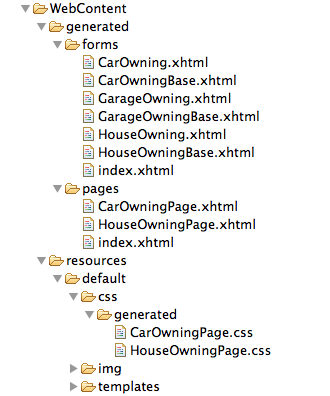
\includegraphics[width=7cm]{./images/chapter03/referenceimpl_projecttree_qls.png}
\end{wrapfigure}

The intended generated file structure is visualized in the screenshot on the
left. The files in the folder \texttt{forms} are generated by the QL model to
code generator as described in chapter \ref{chp:QLCodeGenerator}. The code
generator for the QLS model needs to generate the XHTML files under the folder
\texttt{pages} and the CSS files in \texttt{resources/default/css/generated}.
The file \texttt{pages/index.xhtml} serves as root page containing the link to
the first actual page to be presented.

The page \emph{HouseOwningPage} contains two sections using the forms \emph{HouseOwning} 
and \emph{GarageOwning}, thus the generated file
\texttt{pages/HouseOwningPage.xhtml} composes the two base files
\texttt{forms/HouseOwningBase.xhtml} and \texttt{forms/GarageOwningBase.xhtml}
together: \newline

\begin{lstlisting}[language=HTML]
<html xmlns="http://www.w3.org/1999/xhtml"
      xmlns:ui="http://java.sun.com/jsf/facelets"
      xmlns:h="http://java.sun.com/jsf/html"
      xmlns:f="http://java.sun.com/jsf/core">
  <h:head></h:head>
  <ui:composition template="/index.xhtml">
    <ui:define name="content">
      <h:outputStylesheet library="default/css/generated" name="HouseOwningPage.css"  />
      <div><ui:include src="/generated/forms/HouseOwningBase.xhtml" /></div><p/>
      <div><ui:include src="/generated/forms/GarageOwningBase.xhtml" /></div>
  	  <div>
  	    <h:outputLink value="CarOwningPage.jsf">CarOwningPage</h:outputLink>
  	  </div>
    </ui:define>
  </ui:composition>
</html>
\end{lstlisting}

The two pages are referenced in lines 9 and 10. Line 12 defines the link to the
next page as defined in the \texttt{navigation} section of the QLS model. Line 8
specifies which CSS file is to be used to render the site's elements. The CSS
file for the house owning page contains all corresponding styling information 
which are linked to the corresponding label elements by their ids:

\begin{lstlisting}[language=HTML]
#houseowning\:lblHasBoughtHouse {
	font-style:  italic; 	
}
#houseowning\:lblValueResidue {
	color:       #2233FF; 
	font-family: Verdana; 	
	font-weight: bold; 		
}
#garageowning\:lblHasBoughtGarage {
}
\end{lstlisting}

When JSF converts from XHTML each element gets a unique (full qualified) id. In
our scenario this is always the id of the parent form concatenated with the id
of the elment itself. As separator JSF uses a colon. However, colons are special characters
in CSS, hence they need to be escaped.

Now that the intended artifacts to be generated are clearified, the code generator
itself can be written. Here again we use Xtend (see section \ref{sec:Xtend}):

\begin{lstlisting}[language=Xtend]
class QlsDslGenerator implements IGenerator {
  @Inject extension JsfOutputConfigurationProvider
  @Inject extension QlDslExtensions
  
  override void doGenerate(Resource input, IFileSystemAccess fsa) {
    if (input.URI.fileExtension!="qls")
      return
            
    val styleModel = input.contents.head as QuestionnaireStyleModel
    for (page: styleModel.pages) {
      val cssContent = generateCssFile(page);
   	  val cssFileName = "resources/default/css/generated/"+page.name+".css"
   	  fsa.generateFile(cssFileName, WEB_CONTENT, cssContent)
   	
   	  val xhtmlContent = generateXhtmlFile(page);
   	  val xhtmlFileName = "generated/pages/"+page.name+".xhtml"
   	  fsa.generateFile(xhtmlFileName, WEB_CONTENT, xhtmlContent)
    }
    val contentIndex  = generateIndexPage(styleModel.pages.get(0))
    fsa.generateFile("generated/pages/index.xhtml",WEB_CONTENT, contentIndex)
  }

  def generateCssFile(Page page) '''
  	<!-- @generated -->
    «FOR styleInfo: page.eAllContents.filter(typeof(StyleInformation)).toList»
		«styleInfo.id» {
		  «IF styleInfo.fontColor != null»color: «styleInfo.fontColor»;«ENDIF»
		  «IF styleInfo.fontFamily != null»font-family: «styleInfo.fontFamily»;«ENDIF»
		  «IF styleInfo.fontStyle != null»font-style: «styleInfo.fontStyle»;«ENDIF»
		  «IF styleInfo.fontWeight != null»font-weight: «styleInfo.fontWeight»;«ENDIF»
		}
   «ENDFOR»
  '''
	
  def generateXhtmlFile(Page page) '''
	<!-- @generated -->
	<html xmlns="http://www.w3.org/1999/xhtml"
	      xmlns:ui="http://java.sun.com/jsf/facelets"
	      xmlns:h="http://java.sun.com/jsf/html"
	      xmlns:f="http://java.sun.com/jsf/core">
	  <h:head></h:head>
	  <ui:composition template="/index.xhtml">
	    <ui:define name="content">
	      <h:outputStylesheet library="default/css/generated" name="«page.name».css"  />
	      «IF page.form != null»
	      <div><ui:include src="/generated/forms/«page.form.name»Base.xhtml" /></div>
	      «ELSE»
	        «FOR section: page.eAllContents.toList.filter(typeof(Section)).toList SEPARATOR '<p/>'»
	        <div><ui:include src="/generated/forms/«section.form.name»Base.xhtml" /></div>
	        «ENDFOR»
	      «ENDIF»
	  
	  	  <div>
	  	  «IF page.navigation != null»
	  	    «FOR nextPage: page.navigation.nextPage»
	  	    <h:outputLink value="«nextPage.name».jsf">«nextPage.name»</h:outputLink>
	  	    «ENDFOR»
	  	  «ENDIF»
		  </div>
	    </ui:define>
	  </ui:composition>
	</html>
  '''
    
  def generateIndexPage(Page page)'''
	<?xml version='1.0' encoding='UTF-8' ?>
	<!-- @generated -->
	<!DOCTYPE html PUBLIC "-//W3C//DTD XHTML 1.0 Transitional//EN" "http://www.w3.org/TR/xhtml1/DTD/xhtml1-transitional.dtd">
	<html xmlns="http://www.w3.org/1999/xhtml"
	      xmlns:h="http://java.sun.com/jsf/html"
	      xmlns:ui="http://java.sun.com/jsf/facelets">
	  <ui:composition template="/index.xhtml">
	    <ui:define name="content">
	      <h:outputLink value="«page.name».jsf">«page.name»</h:outputLink>
	    </ui:define>
	  </ui:composition>
	</html>
  '''	
	
  def getId(StyleInformation styleInfo) {
    val question = (styleInfo.eContainer as QuestionStyling).question
    "#"+question.form.id+ "\\:lbl"+question.id.toFirstUpper
  }
}
\end{lstlisting}

The \texttt{doGenerate} method is similar to the one of the
\texttt{JSFGenerator} from section \ref{sec:jsfGenerator}. It basically defines
file names and delegates to other methods for defining the generated files'
contents (\texttt{generateCssFile}, \texttt{generateXhtmlFile},
\texttt{generateIndexPage}). We won't go into details here. Instead let's test
the generated application.
